\documentclass[11pt]{article}
\usepackage{acl2014}
\usepackage{times}
\usepackage{url}
\usepackage{latexsym}
\usepackage{hyperref}
\usepackage{graphicx}
\usepackage{booktabs} 

\title{Music recommendations}

\author{Sergio Kazatzidis \\
    {\tt s.kazatzidis@gmail.com} \\
    Kamiel Fokkink \\
    {\tt kamielfokkink@gmail.com} \\\And
    Baran İşcanlı \\
    {\tt barantevitol@gmail.com} \\
    Tomas Kehus \\
    {\tt tekehus@gmail.com}}

\date{24/12/2019}

\begin{document}
\maketitle
\begin{abstract}
    Recommender systems are used to predict recommendations for a user based on previous behaviour, that will match the users preferences and interests. The goal of this project is to build two recommender systems, based on two common approaches: user based and content based recommendations. The machine learning principle behind these models is k Nearest Neighbours, which looks at the k most similar datapoints to a target point. Our model was evaluated by using the mean absolute error, because of its simplicity and popularity among other recommender system builders. The created recommender system worked best when using cosine similarity and the number of items in the neighbourhood,k,was big. And when it only had to recommend few items.
\end{abstract}

\noindent

\section{Introduction}
Recommender systems are a set of techniques used to recommend new products to a user, and are widely used in industries that provide consumer products. Netflix uses it for recommending movies to its users, Facebook for building of a newsfeed, and Youtube recommends videos that its users might want to view. The algorithm tries to predict recommendations for users that are likely to match their needs or interests, based on their previous purchasing or viewing patterns. They rely on large amounts of data that track patterns in peoples' behaviour, to build up a profile of the user, and be able to predict a meaningful recommendation. There are two main ways to approach this problem. Collaborative filtering looks at relationships and similarities between users, and content based filtering looks at relationships between items. Many industrial implementations make use of a hybrid version that combines elements of the two. Our goal for this project is to create recommender systems for amazon customers, based on their previous purchases and ratings. It will build a model for the two types of recommendations, those based on user-to-user, and item-to-item. \\

\section{Dataset}
The dataset that we used for the training of our model was Amazon review data, which was retrieved from \href{http://jmcauley.ucsd.edu/data/amazon/}{here}. This database contains review information about numerous kinds of products, ranging from groceries to clothes to video games. But reviews about for example kitchen appliances would say more about the quality of the product, and not about a consumers individual tastes. The most suitable kinds of products to train a recommender system on are those of which the review reflects the particular persons interests and tastes. Therefore, we chose to use the datasets of Kindle books, video games, and digital music. The database offers two options for the dataset: all aggregated reviews, or a filtered dataset to only include reviewers that rated 5 or more products. We chose the second option, because it reduces the cost of training, and it is more relevant to have several datapoints per user, so as to have more information for good recommendations. \\

\subsection{Splitting the data}
The sizes of the datasets are: 31MB and 64k lines for the music, 110MB and 231k lines for the video games, and 266MB and 982k lines for the books. For each review, there are several features that we can include. Some are necessary for our analysis, such as the reviewer ID, product ID, and the review score. Many features are also less relevant for our purposes, but can be included if needed, such as the review time or a review text. A printout sample of the data can be seen in figure 1. \\
\begin{figure}
    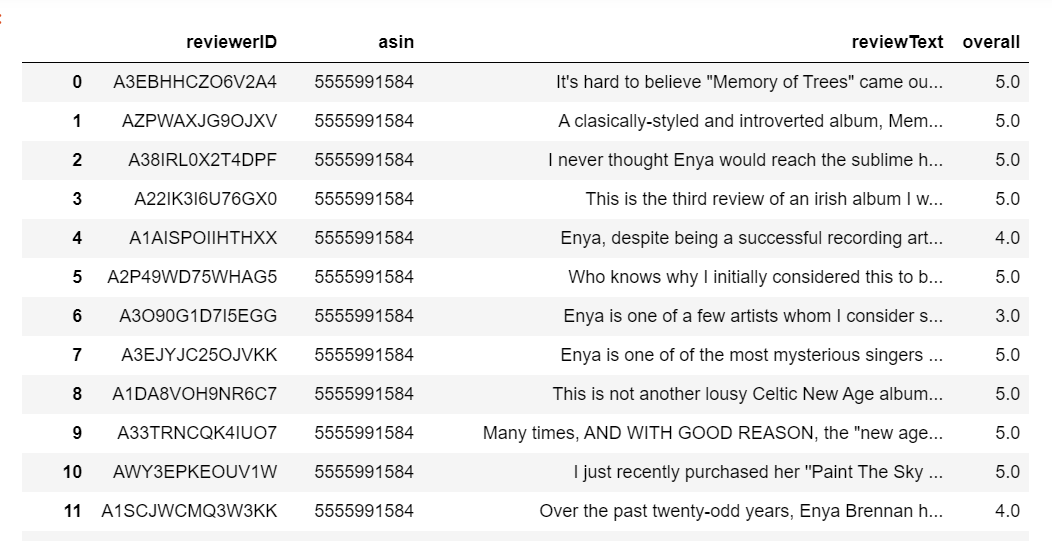
\includegraphics[width=7.5cm]{Pandas_df_example.png}
    \caption{Pandas dataframe of the data}
\end{figure}

For testing purposes, we want to split our data into a training and a testing set. This is not just a simple randomized split of the datapoints. For the evaluation of our recommender system, we need to split our user base, taking out 10\% of all users and putting them in a test set. Our test set will therefore consist of completely new users who have not been used for the training of our model. By looking at a few of those new user's preferences, the model can then recommend them new items to buy. We will be able to compare these recommendations to our expected recommendations, to evaluate our model.

\section{k-NN}
K-nn classification is a simple concept, where a point is given the same class as the nearest k points around it. The value of k is a hyperparameter, which has to be provided beforehand. In our case, we will try out different values for k, to find out which one has the optimal performance. K-nn has the advantages of speed and minimal necessary processing power. It also requires no training time- this can potentially be seen as a negative aspect, as there is no 'learning' within a model. However, our dataset has enough datapoints that it should be able to provide reliable recommendations, even with such a simple algorithm. We chose two different techniques to implement K-nn: user-to-user, and item-to-item.
\subsection{User-to-user}
User-to-user is a technique to suggest items to a user. When used with a K-nn classifier, it assesses the similarities of a given user $U$ to other users. Then, it predicts how would $U$ have rated the items in lists of similar users, filtering the items $U$ has already rated. By doing so, a ranking between items are created. Afterwards the top $n$ items are recommended to the user, $n$ being an arbitrary number. Basic steps can be outlined as such:
\begin{enumerate}
	\item Find the similarities of the given user $U$ to every other user, based on the items they all rated.
	\item Rank the top $K$ similar users to create a $neighborhood$ for the user.
	\item For every item in the neighborhood that has not been rated by $U$, get a rating prediction. The prediction is based on the formula $$r_{predict}=\frac{1}{N\times\sum_{j=0}^{N}s_i}\sum_{i=0}^{N}r_i\times s_i$$N being the total number of neighbors that used the item
\end{enumerate}
The method stated above is successful in an abundant and dense dataset. However, since our dataset was significantly sparse, we hypothesized that this method will be affected a lot. Thus, we modify the $3^{rd}$ step. Instead of using the similarities as weight, we look at the intersection of shared rated items between the two users. This approach is recommended by \footnote[1]{https://towardsdatascience.com/introduction-to-recommender-systems-6c66cf15ada}, as our data is sparse, and most items will not have been rated by both users. From the intersection of shared items, we compute the similarity between two users' ratings of those items. However, just this similarity is not enough, it needs to be weighted. If a target user made twenty reviews, and shares just one item with another user, for which they gave the same rating, it would give a similarity of 1. This is obviously not the case, as the target user has rated 19 other items as well. Therefore, we weight the similarity with length of the set of shared items, divided by the total amount of items rated by the target user.. 

\subsection{Item-to-item}
Item-to-item, is another technique that we implemented. Rather than basing the similarities on users, it utilizes the item similarities. The steps of this technique are:
\begin{enumerate}
	\item Find all the similarities between each item pair
	\item Created $neighborhoods$ of size $K$, which means an item $I$ should be listed with all the top $K$ similar items, along with their similarity rate to $I$.
	\item Finally, for the user $U$, it predicts the rating given by the user. To predict the rating, same formula is used. However, the similarity measures are now item-to-item similarity
\end{enumerate}
For this technique, we wanted to keep the original formula, to see if our hypothesis was actually true, and the predictions would not be as accurate as the user-to-user approach. Therefore, out item-to-item approach gave predicted ratings as well as a list of ranked items.


\subsection{Similarity measures}
There are several ways to calculate the similarity between two users. A user is represented by a vector, where each entry is the users interaction with a product. These vectors are sparse, with most of the entries set to 0, as the user does not interact with most of the items. The other entries contain the users rating for that product, between 1 to 5. There are three similarity measures that we consider, and during the development phase we see which of these measures performs best. The first is Euclidean similarity, which is the inverse of the Euclidean distance of the points in space. The second is cosine similarity, which is the dot product of the two vectors scaled by their length, thus giving the angle between the vectors. The third is pearson correlation, a measure of the strength of linear dependence between two vectors. Because we only computed the similarity between the shared items, we need to weigh this similarity. If two users would have one item in common for which they both gave a 5.0, their similarity would be 1.0, but indeed they are quite different in their preferences. So we weigh the similarity by multiplying it with the size of their shared items divided by the amount of items reviewed by the target user.
\section{Evaluation}
Evaluating a recommender system is a difficult task, but an important one. It is of great significance for the development of the system. While having multiple evaluations to choose from, to pick the best one among them given the situation is still a problem with no definite solution (Lü et al., 2012).  The classical approach for evaluating a recommender system is by splitting the data arbitrarily into training data and test data. However, according to Said, Bellogin & Kouki (2013) this is not the best method to evaluate the recommender system. They apply a different method where they try to mimic the data attributes of already used recommender systems, such as Netflix, by splitting the training data and test data more realistically, however this is out of the scope of this paper. There are multiple ways to measure the accuracy of a recommender system. Two method that are often used, because of their simplicity are the Mean Absolute Error and the Root Mean Squared Error. This is utilized to see whether the predicted rating is close to the actual rating the user gave to a certain product. \\
\m
$$MAE =  (\frac{1}{n})\sum_{i=1}^{n}\left | y_{i} - x_{i} \right |\\ $$\\
\\$$RMSE=\sqrt{(\frac{1}{n})\sum_{i=1}^{n}(y_{i} - x_{i})^{2}} $$

Where n is the set of user ratings on other products. And y(i) is the predicted rating and x(i)  the true rating. 
If the values of these two errors is low, it means that the recommender system has a high accuracy (Lü et al., 2012). Another way to evaluate, when there are no predicted scores available, is to look at the overlap between the predicted items and the 'true' items.


\section{Results}
\subsection{Item-item classification}
The accuracy of the recommender system that was based on item to item classification has been evaluated with the Mean Absolute Error. The variables that were being varied were the k, number of items in a neighborhood, and the different kind of similarities. The cosine similarity had the lowest cost when k = 100. Namely, a cost of roughly 3.395.In Table 1 the results of this will be shown.\\ 


\begin{table}[h]
	
	\begin{tabular}{@{}|l|l|l|l|@{}}
		\toprule
		& Euclidean & Cosine & Pearson \\ \midrule
		Cost & 3.79659              & 3.39459           & 5.21993             \\ \bottomrule
	\end{tabular}
	\caption{Costs of different similarity measures}
\end{table}
\newpage
After this the k, items in the neighborhood, was varied, while using the cosine similarity measurement (see Table 2). The best one was k = 100 with a cost of 3.39459.

\begin{table}[h]
	\begin{tabular}{@{}ll@{}}
		\toprule
		k   & Cost    \\ \midrule
		5   & 5.39197 \\
		10  & 4.90762 \\
		20  & 4.37366 \\
		50  & 3.98604 \\
		100 & 3.39459 \\ \bottomrule
	\end{tabular}
	\caption{Costs of different k when using cosine similarity measures}
\end{table}

\subsection{User-user classification}
The accuracy of the recommender system that was based on user to user classification has been evaluated in a different way than the Mean Absolute Error. Instead we will look at the ratio of the predicted items and that were already bought by the user. We varied the k, amount of items in a neighbourhood, and n, the amounts of items that were recommended. The predicted recommendations were based on 80 percent of each test-user's data.

% Please add the following required packages to your document preamble:
% \usepackage{booktabs}
\begin{table}[h]
	\begin{tabular}{@{}|l|l|l|l|l|@{}}
		\toprule
		\begin{tabular}[c]{@{}l@{}}n\\ k\end{tabular} & 5 & 10 & 20 & 35 \\ \midrule
		5 & 1,103 & 0,898 & 0,657 & 0,513 \\ \midrule
		10 & 0,907 & 0,649 & 0,603 & 0,435 \\ \midrule
		20 & 0,369 & 0,312 & 0,255 & 0,1844 \\ \midrule
		50 & 0,517 & 0,414 & 0,372 & 0,260 \\ \midrule
		100 & 0,481 & 0,412 & 0,271 & 0,187 \\ \bottomrule
	\end{tabular}
	\caption{Overlap of recommended items with purchased items in percentage.}
\end{table}

\part{title}
\subsection{Conclusion and Discussion}
Our project was successful in creating a recommender system, which provided recommendations, based on our own internal algorithms. Our biggest issues were in creating evaluation metrics and functions, as well as dealing with our large quantities of data. We found that the User-to-User system was easier to implement, requiring less processing, and working better in areas of our dataset with low information density. This is quite normal, for both types of systems, working with the same dataset. However, both methods have value in making item recommendations, and they could be used collaboratively for best results. This would allow a recommender system to use the strengths of each system, based on similarities between users and items. If we were to take this project further, it would be very interesting to be able to use more data, such as more detailed user information. This could possibly include demographics, searches, viewing and clicking data, and more.
 

\section{Bibliography}
Herlocker, J., Konstan, J., Terveen, L., & Riedl, J. (2004). Evaluating collaborative filtering recommender systems. ACM Transactions on Information Systems (TOIS), 22(1), 5–53. https://doi.org/10.1145/963770.963772

Lü, L., Medo, M., Yeung, C., Zhang, Y., Zhang, Z., & Zhou, T. (2012). Recommender systems. Physics Reports, 519(1), 1–49. https://doi.org/10.1016/j.physrep.2012.02.006

Said, A., Bellogín Kouki, A., Vries, A., & Information Access. (2013). A Top-N Recommender System Evaluation Protocol Inspired by Deployed Systems.

\end{document}
